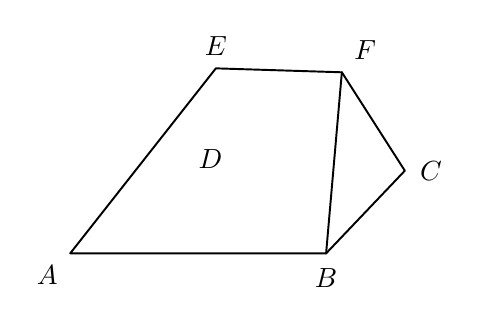
\begin{tikzpicture}[line join=round, line cap=round]
  \coordinate (A) at (0,0);
  \coordinate (B) at (3.25,0);
  \coordinate (C) at (4.25,1.05);
  \coordinate (E) at (1.85,2.35);
  \coordinate (F) at (3.45,2.30);

  \draw[line width=0.7pt] (A)--(B)--(C)--(F)--(E)--cycle;
  \draw[line width=0.7pt] (B)--(F);

  \node[below left=1pt] at (A) {$A$};
  \node[below=2pt] at (B) {$B$};
  \node[right=2pt] at (C) {$C$};
  \node[above=1pt] at (E) {$E$};
  \node[above right=1pt] at (F) {$F$};
  \node at (1.78,1.20) {$D$};
\end{tikzpicture}
